\documentclass{article}
\usepackage{amsmath}
\usepackage[mathletters]{ucs}
\usepackage[utf8x]{inputenc}
\usepackage[margin=1.5in]{geometry}
\usepackage{enumerate}
\newtheorem{theorem}{Theorem}
\usepackage[dvipsnames]{xcolor}
\usepackage{pgfplots}
\pgfplotsset{compat=1.18}
\setlength{\parindent}{0cm}
\usepackage{graphics}
\usepackage{graphicx} % Required for including images
\usepackage{subcaption}
\usepackage{bigintcalc}
\usepackage{pythonhighlight} %for pythonkode \begin{python}   \end{python}
\usepackage{appendix}
\usepackage{arydshln}
\usepackage{physics}
\usepackage{booktabs} 
\usepackage{adjustbox}
\usepackage{tikz}
\usepackage[framemethod=tikz]{mdframed}
\usepackage{relsize}
\usepackage{physics}
\usepackage[thinc]{esdiff}
\usepackage{esint}  %for lukket-linje-integral
\usepackage{xfrac} %for sfrac
\usepackage[colorlinks=true]{hyperref} %for linker, må ha med hypersetup
\usepackage[noabbrev, nameinlink]{cleveref} % to be loaded after hyperref
\usepackage{amssymb} %\mathbb{R} for reelle tall, \mathcal{B} for "matte"-font
\usepackage{listings} %for kode/lstlisting
\usepackage{verbatim}
\usepackage{graphicx,wrapfig,lipsum,caption} %for wrapping av bilder
\usepackage{mathtools} %for \abs{x}
\usepackage[norsk]{babel}
\usepackage{cancel}
\definecolor{codegreen}{rgb}{0,0.6,0}
\definecolor{codegray}{rgb}{0.5,0.5,0.5}
\definecolor{codepurple}{rgb}{0.58,0,0.82}
\definecolor{backcolour}{rgb}{0.95,0.95,0.92}
\lstdefinestyle{mystyle}{
    backgroundcolor=\color{backcolour},   
    commentstyle=\color{codegreen},
    keywordstyle=\color{magenta},
    numberstyle=\tiny\color{codegray},
    stringstyle=\color{codepurple},
    basicstyle=\ttfamily\footnotesize,
    breakatwhitespace=false,         
    breaklines=true,                 
    captionpos=b,                    
    keepspaces=true,                 
    numbers=left,                    
    numbersep=5pt,                  
    showspaces=false,                
    showstringspaces=false,
    showtabs=false,                  
    tabsize=2
}

% Create a command for creating a simple box with support for equations with transparent background



\newcommand{\boks}[1]
{
  \begin{center}
  \begin{mdframed}
  {#1}
  \end{mdframed}
  \end{center}
}


\lstset{style=mystyle}
\author{15033}
\title{Midterm}
\date{}
\begin{document}
\maketitle


\section*{a)}
The possible eigenvalues of the Hamiltonian is the possible values of the sum of the eigenvalues of the operators its made of. 
\begin{align}
\hat{H} = \frac{α}{ℏ} \vec{L}^2 + β \hat{L}_z
\end{align}
Applying the operators on an arbitrary eigenstate $\ket{m,l}$ we get:
\begin{align}
\hat{L}_z \ket{m,l} = m ℏ \ket{m,l}
\end{align}
\begin{align}
\vec{L}^2 \ket{m,l} = l(l+1) ℏ^2 \ket{m,l}
\end{align}
The eigenvalues are clearly $m ℏ$ and $l(l+1) ℏ^2$ for $\hat{L}_z$ and $\vec{L}^2$ respectively.

As the operators act linearly, we know the possible eigenvalues of each operator and can therefore just write out the sum as follows:
\begin{align}
\underline{\underline{E_{l,m} = α ℏl(l+1) + β ℏ m}}
\end{align}
When $β = 0$, we know the ten lowest energy eigenvalues are degenerate for different values of $m$. The nine lowest energy eigenvalues are therefore the energies of $l ∈ [0,1,2]$ with $m ∈ [-l, -l+1, ..., l-1, l]$. We get the 10'th value for $l = 3$, with $m = -l$ . Plotting this for a $β / α$ ratio from 0, to 8 we get \cref{fig: a}.

\begin{figure}[h!]
\centering
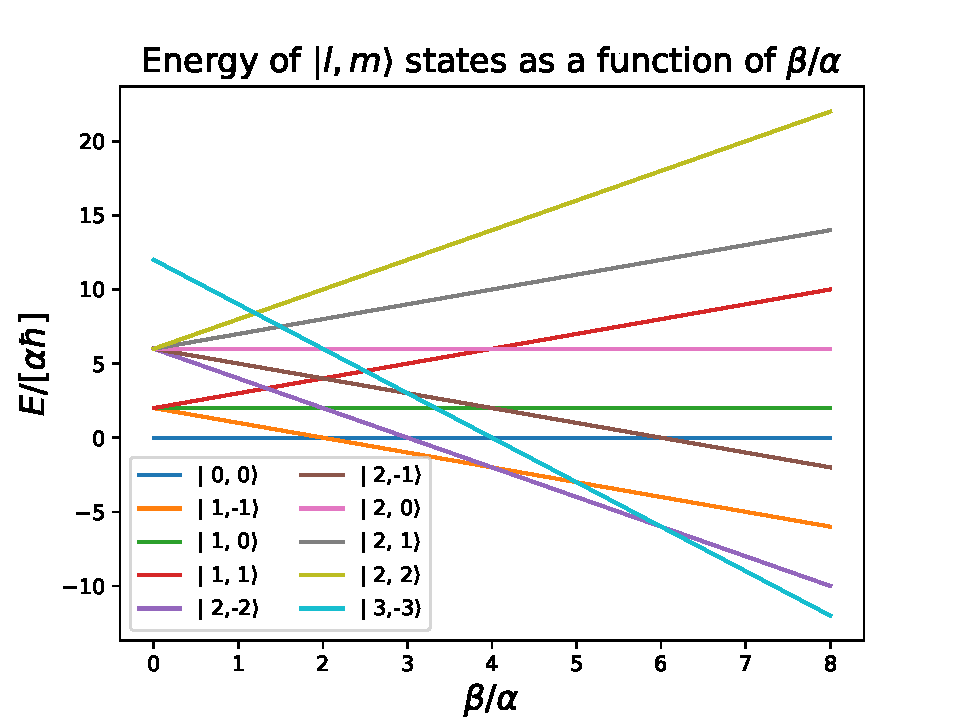
\includegraphics[width = .65\textwidth]{a.pdf}
\caption{Plot of the ten lowers energy eigenvalues as a function of $β / α$.}
\label{fig: a}
\end{figure}

\section*{b)}

The ground state is the lowest possible energy state. We can therefore iterate over different $l$ and $m$-values and plot the $\hat{L}_z$-expectation values as a function of $β / α$ to find the ground state.
\begin{align}
ψ_0 = \ket{l,m}
\end{align}
\begin{align}
\bra{ψ_0}L_z\ket{ψ_0} = mℏ 
\end{align}
Defining the ratio $γ = β / α$, we can extrapolate from the plot in \cref{fig: a}, that the lowest energy eigenvalue belongs to the state $\ket{l, -l}$ for $l = \operatorname{floor}\left(γ / 2\right)$. At the exact point where $γ = 2n \ , \  n ∈ [1,2,3, \ldots]$ the ground state is degenerate for $m = -l$ for both $l_1 = \operatorname{floor}(γ / 2)$ and $l_2 = l_1 - 1$. The angular momentum of the lowest energy state is visualized in \cref{fig: b}. The scatter point show the degenerate ground states. 

\begin{figure}[h!]
\centering
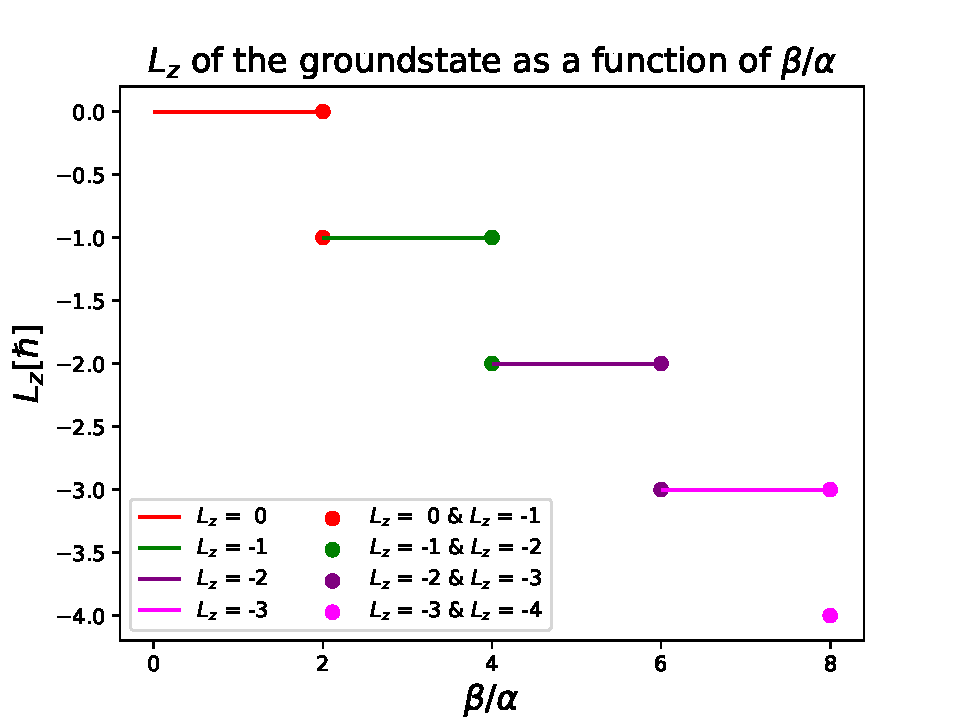
\includegraphics[width = .65\textwidth]{b.pdf}
\caption{Angular momentum in the $z$-direction of the ground state as a function of $β / α$. Scatterpoints shows the angular momentum for degenerate ground states.}
\label{fig: b}
\end{figure}

\section*{c)}
We know the time evolution of a sate $\ket{ψ(t)}$ is given by:
\begin{align}
\ket{ψ(t)} = e^{-i \hat{H} t / ℏ} \ket{ψ(0)}
\end{align}
Adding our Hamiltonian to the time evolution operator, we get:
\begin{align}
\ket{ψ(t)} = e^{-i \left(\frac{α}{ℏ} \vec{L}^2 + β \hat{L}_z\right) t / ℏ} \ket{ψ(0)}
\end{align}
To make this easier to deal with, we can write the exponential as the product of two exponentials:
\begin{align}
e^{-i \left(\frac{α}{ℏ} \vec{L}^2 + β \hat{L}_z\right) t / ℏ} = e^{-i \frac{α}{ℏ} \vec{L}^2 t / ℏ} e^{-i β \hat{L}_z t / ℏ}
\end{align}
Beginning with the first exponential, we can rewrite the expression as a Taylor series:
\paragraph{First: }
\begin{align}
e^{-i \frac{α}{ℏ} \vec{L}^2 t / ℏ} \ket{ψ(0)} = \Bigg(\frac{1}{0!} -\frac{1}{1!}i t\frac{α}{ℏ^2}\vec{L}^2 + \frac{1}{2!} \left(t\frac{α}{ℏ^2}\vec{L}^2\right)^2 + \ldots\Bigg)\ket{ψ(0)}
\end{align}
We know the operator acting on the state $\ket{ψ(0)}$ returns the eigenvalue of the operator times the state. All the states in the superposition have the same $l$-value. We therefore get:
\begin{align}
e^{-i \frac{α}{ℏ}\vec{L}^2 t / ℏ} \ket{ψ(0)} = \Big( 1 -2iαt + \frac{1}{2!} 4αt + \ldots\Big) \ket{ψ(0)}
\end{align}
The pattern is clear, and we can write this back as an exponential:
\begin{align}
\underline{e^{-2iαt} \ket{ψ(0)}}
\end{align}

\paragraph{Sedond: }
\begin{align}
e^{-i β \hat{L}_z t / ℏ} \ket{ψ(0)} = \Bigg(\frac{1}{0!} -\frac{1}{1!}i t\frac{β}{ℏ}\hat{L}_z + \frac{1}{2!} \left(t\frac{β}{ℏ}\hat{L}_z\right)^2 + \ldots\Bigg)\ket{ψ(0)}
\end{align}
The $L_z$ operator acts differently on all the kets in the superposition. We can therefore write:
\begin{align}
\hat{L}_z \ket{1,-1} = -ℏ \ket{1,-1}
\end{align}
\begin{align}
\hat{L}_z \ket{1,0} = 0 \ket{1,0}
\end{align}
\begin{align}
\hat{L}_z \ket{1,1} = ℏ \ket{1,1}
\end{align}
Expanding the state vector and applying the $L_z$ operator, we get:
\begin{align}
\underline{e^{-i β \hat{L}_z t / ℏ} \ket{ψ(0)} = \frac{1}{2} e^{iβt}\ket{1,-1} + i\sqrt{2} \ket{1,0} - \frac{1}{2} e^{-iβt}\ket{1,1}}
\end{align}
\paragraph{Combining the Results: }
\begin{align}
\underline{\underline{\ket{ψ(t)} = \frac{1}{2} e^{-2iαt} \left(e^{iβt}\ket{1,-1} + i\sqrt{2} \ket{1,0} - e^{-iβt}\ket{1,1}\right)}}
\end{align}

\paragraph{Expectation Value: }
\begin{align}
\left<\hat{L}_z(t)\right> = \bra{ψ(t)} \hat{L}_z \ket{ψ(t)}
\end{align}
\begin{align}
\left<\hat{L}_z(t)\right> = \bra{ψ(t)} \Bigg( \frac{ℏ}{2} e^{-2ia} \Big(-e^{iβt}\ket{1,-1} + e^{-iβt}\ket{1,1}\Big) \Bigg)
\end{align}
\begin{align}
\underline{\underline{\left<\hat{L}_z(t)\right> = \frac{ℏ}{2} - \frac{ℏ}{2} = 0 }} 
\end{align}

\section*{d)}
The possible eigenvalues of the $\hat{L}_z$ operator is still $ℏm$, as the superposition is made of the eigenstates of $\hat{L}_z$. 
\begin{align}
P(L_z = -ℏ)  = \left|\bra{1,-1}\ket{ψ(t)}\right|^2 = \left|\frac{1}{2} e^{-2iαt} e^{iβt}\right|^2
\end{align}
\begin{align}
\underline{\underline{P(L_z = -ℏ) = \frac{1}{4}}}
\end{align}
\begin{align}
P(L_z = 0) = \left|\bra{1,0}\ket{ψ(t)}\right|^2 = \left|\frac{1}{2}e^{-2iαt} i \sqrt{2}\right|^2 
\end{align}

\begin{align}
\underline{\underline{P(L_z = 0) = \frac{1}{2}}}
\end{align}

\begin{align}
P(L_z = ℏ) = \left|\bra{1,1}\ket{ψ(t)}\right|^2 = \left|\frac{1}{2} e^{-2iαt} e^{-iβt}\right|^2
\end{align}
\begin{align}
\underline{\underline{P(L_z = ℏ) = \frac{1}{4}}}
\end{align}

Summing the values together with their respective probabilities, we get:
\begin{align}
\underline{\underline{\left<\hat{L}_z(t)\right> = -ℏ \frac{1}{4} + 0 \frac{1}{2} + ℏ \frac{1}{4} = 0}}
\end{align}

\newpage
\section*{e)}
\boks{
  \subsection*{Definitions:}
  \begin{align} \label{trig_id}
  2i \sin θ = e^{iθ} - e^{-iθ}
  \end{align}
  \begin{align}
    \hat{L}_x = \frac{1}{2} \left(\hat{L}_+ + \hat{L}_-\right)
  \end{align}
  \begin{align}
    \hat{L}_+ \ket{l,m} = ℏ \sqrt{l(l+1) - m(m+1)}\ \ket{l,m+1} = ℏ\sqrt{(l-m)(l+m+1)}\ \ket{l,m+1}
  \end{align}
  \begin{align}
    \hat{L}_- \ket{l,m} = ℏ \sqrt{l(l+1) - m(m-1)}\ \ket{l,m-1} = ℏ\sqrt{(l+m)(l-m+1)}\ \ket{l,m-1}
  \end{align}
  }
  Before finding the expectation value, we see how the operator acts on our kets:
  \boks{
    \subsection*{Action on Kets:}
    \begin{equation*}
      \begin{aligned}[c]
        \hat{L}_{+} \ket{1,-1} &= \sqrt{2}ℏ \ket{1,0}  \\ 
        \hat{L}_{+} \ket{1,\ \ 0} &= \sqrt{2}ℏ \ket{1,\ \ 1} \\ 
        \hat{L}_{+}\ket{1,\ \ 1} &= 0
      \end{aligned}\quad \vline \quad 
      \begin{aligned}[c]
        \hat{L}_{-} \ket{1,-1} &= 0\\ 
        \hat{L}_{-} \ket{1,\ \ 0} &= \sqrt{2}ℏ \ket{1,-1} \\ 
        \hat{L}_{-}\ket{1,\ \ 1} &= \sqrt{2}ℏ \ket{1,0}
      \end{aligned}
    \end{equation*}
    }
\subsection*{$\bf \hat{L}_x$:}
  Having done this, we can find its expectation value as follows:
\begin{align}
\left<\hat{L}_x\right> = \bra{ψ(t)} \hat{L}_x \ket{ψ(t)} = \bra{ψ(t)} \frac{1}{2} \left(\hat{L}_+ + \hat{L}_-\right) \ket{ψ(t)}
\end{align}
\begin{align}
\left<\hat{L}_x\right> = \frac{1}{2} \bra{ψ(t)} \left(L_+ \ket{ψ(t)} + L_-\ket{ψ(t)}\right)
\end{align}
\begin{align}\label{eq: L_x psi}
\left<\hat{L}_x\right> = \frac{1}{2} \frac{1}{2}e^{-2iαt} \bra{ψ(t)} \left(\sqrt{2}ℏe^{iβt}\ket{1,0} + 2iℏ\ket{1,-1} + 2iℏ\ket{1,1} - \sqrt{2}ℏe^{-iβt}\ket{1,0}\right) 
\end{align}
Using the orthonormality of the eigenstates, we can write:
\begin{align}
\left<\hat{L}_x\right> = \frac{1}{8}\Big( -2iℏe^{iβt} -  2iℏe^{iβt} + 2iℏe^{-iβt} + 2iℏe^{-iβt jj } \Big)
\end{align}
\begin{align}
\left<\hat{L}_x\right> = -\frac{1}{2}ℏi \left(e^{iβt} - e^{-iβt}\right)
\end{align}
Using \cref{trig_id} we can rewrite this as: 
\begin{align}
\underline{\underline{\left<\hat{L}_x\right> = ℏ\sin(βt)}}
\end{align}

\subsection*{$\bf \hat{L}^2_x$:}
% When calculating the expectation value of this operator squared, we will many terms because of the way we defined the $\hat{L}_x$. Rewriting our state vector in the $\hat{L}_x$ basis, we get:

We continue from \cref{eq: L_x psi} from the previous problem, before we took the inner product:

\begin{align}\label{eq: full}
\frac{1}{4}e^{-2iαt} \bra{ψ(t)} \hat{L}_x \left(\sqrt{2}ℏe^{iβt}\ket{1,0} + 2iℏ\ket{1,-1} + 2iℏ\ket{1,1} - \sqrt{2}ℏe^{-iβt}\ket{1,0}\right)
\end{align}

Just looking at how the operator acts on the kets, we begin with:

\begin{align}
\frac{1}{2}\left(\hat{L}_+ + \hat{L}_-\right) \left(\sqrt{2}ℏe^{iβt}\ket{1,0} + 2iℏ\ket{1,-1} + 2iℏ\ket{1,1} - \sqrt{2}ℏe^{-iβt}\ket{1,0}\right)
\end{align}

\begin{align}
ℏ^2e^{iβt} \ket{1,1} + ℏ^2e^{iβt} \ket{1,-1} + \sqrt{2}iℏ^2 \ket{1,0} + \sqrt{2}iℏ^2 \ket{1,0} - ℏ^2e^{-iβt}\ket{1,-1} - ℏ^2e^{-iβt}\ket{1,1}
\end{align}
This can be shortened to:

\begin{align}
ℏ^2\Bigg(e^{iβt}\Big(\ket{1,1} + \ket{1,-1}\Big) + 2\sqrt{2}i\ket{1,0} - e^{-iβt}\Big(\ket{1,1} + \ket{1,-1}\Big) \Bigg)
\end{align}
Agin we use \cref{trig_id} to rewrite this as:  
\[
ℏ^2 \Bigg( 2i\sin (βt) \Big(\ket{1,1} + \ket{1,-1}\Big) + 2\sqrt{2}i \ket{1,0} \Bigg)
\]

Now we can add this back into \cref{eq: full} again:

\begin{align}
\frac{1}{4}ℏ^2 e^{-2iαt} \bra{ψ(t)}\Bigg( 2i\sin (βt) \Big(\ket{1,1} + \ket{1,-1}\Big) + 2\sqrt{2}i \ket{1,0} \Bigg)
\end{align}

\begin{align}
\frac{1}{4}ℏ^2 \Bigg(2i \sin(βt) \left(e^{-iβt} - e^{iβt}\right) + 2\Bigg)
\end{align}

Taking out some factors and using \cref{trig_id} we get:
\begin{align}
\underline{\underline{\left<\hat{L}_x^2\right> = \frac{1}{2}ℏ^2 \Big(\sin^2(βt) + 1\Big)}}
\end{align}


% \begin{align}
% \frac{1}{4}ℏ^2e^{-2iαt} \bra{ψ(t)}\Bigg(e^{iβt}\Big(\ket{1,1} + \ket{1,-1}\Big) + 2\sqrt{2}i\ket{1,0} - e^{-iβt}\Big(\ket{1,1} + \ket{1,-1}\Big) \Bigg)
% \end{align}

% \begin{align}
% \frac{1}{8}ℏ^2\Big( 1 - e^{-2iβt} + 4 + e^{2iβt} - 1\Big)
% \end{align}

% \begin{align}
% \frac{1}{8}ℏ^2 \left(4 + e^{2iβt} - e^{-2iβt}\right)
% \end{align}

% Using \cref{trig_id} we can rewrite this as:

% \begin{align}
% \frac{1}{2}ℏ^2 + \frac{1}{4}i\sin(2βt) ℏ^2
% \end{align}


\section*{f)}
\begin{align}
\frac{ℏ^2}{2} (\sin^2 (βt) + 1)
\end{align}
To find the probabilities of the different eigenvalues when measuring in the $x-$direction, we write the eigenstates of the $\hat{L}_x$ operator in the $z$-basis:
\begin{align}
\ket{1,0}_x = \frac{1}{\sqrt{2}}\Big(\ket{1,1} - \ket{1,-1}\Big)
\end{align}
\begin{align}
\ket{1,1}_x = \frac{1}{2}\ket{1,1} + \frac{\sqrt{2}}{2}\ket{1,0} + \frac{1}{2}\ket{1,-1}
\end{align}
\begin{align}
\ket{1,-1}_x = \frac{1}{2}\ket{1,1} - \frac{\sqrt{2}}{2}\ket{1,0} + \frac{1}{2}\ket{1,-1}
\end{align}

To find the probabilities, we must take absolute value of the projection:

\subsection*{$\underline{\bf P(L_x = ℏ)}$:}
\begin{align}
P(L_x = ℏ) = \left|\bra{1,1}_x\ \ket{ψ(t)}\right|^2
\end{align}
We begin by looking at the inner product first. 
\begin{align}
\Bigg(\frac{1}{2} \bra{1,1} + \frac{\sqrt{2}}{2} \bra{1,0} + \frac{1}{2}\bra{1,-1}\Bigg) \frac{1}{2} e^{-2iαt} \Bigg(e^{iβt}\ket{1,-1} + i \sqrt{2}\ket{1,0} - e^{-iβt}\ket{1,1}\Bigg)
\end{align}
\begin{align}
\frac{1}{4}e^{-2iαt} \Big( e^{iβt} + 2i -e^{-iβt} \Big)
\end{align}
Again we use \cref{trig_id} to rewrite this as:
\begin{align}
\frac{1}{2}e^{-2iαt} \left(\sin (βt) + 1\right)
\end{align}
Taking the absolute value squared, we get:
\begin{align}
\left|\frac{1}{2}e^{-2iαt} \left(\sin (βt) + 1\right)\right|^2
\end{align}

\begin{align}
\underline{\underline{P(L_x = ℏ) = \frac{1}{4} \left(\sin (βt) + 1\right) ^2}}
\end{align}

\subsection*{$\underline{\bf P(L_x = -ℏ)}$:}
\begin{align}
P(L_x = -ℏ) = \left|\bra{1,-1}_x\ \ket{ψ(t)}\right|^2
\end{align}
\begin{align}
\Bigg(\frac{1}{2} \bra{1,1} - \frac{\sqrt{2}}{2} \bra{1,0} + \frac{1}{2}\bra{1,-1}\Bigg) \frac{1}{2} e^{-2iαt} \Bigg(e^{iβt}\ket{1,-1} + i \sqrt{2}\ket{1,0} - e^{-iβt}\ket{1,1}\Bigg)
\end{align}

The only difference from the previous problem is the minus sign in front of the $\sqrt{2}$ term. This only switches the sign in the imaginary number, and we thus get the following:
\begin{align}
\underline{\underline{P(L_x = -ℏ) = \frac{1}{4} \left(\sin (βt) - 1\right)^2 }}
\end{align}

\subsection*{$\underline{\bf P(L_x = 0)}$:}
\begin{align}
P(L_x = 0) = \left|\bra{1,0}_x\ \ket{ψ(t)}\right|^2
\end{align}
Again we focus on the inner product:
\begin{align}
\Bigg(\frac{1}{\sqrt{2}} \bra{1,1} - \frac{1}{\sqrt{2}} \bra{1,-1}\Bigg) \frac{1}{2} e^{-2iαt} \Bigg(e^{iβt}\ket{1,-1} + i \sqrt{2}\ket{1,0} - e^{-iβt}\ket{1,1}\Bigg)
\end{align}
\begin{align}
\frac{\sqrt{2}}{4}e^{-2iαt} \left(- e^{iβt} - e^{-βt}\right)
\end{align}
We use \cref{trig_id} to rewrite this as:
\begin{align}
- \frac{\sqrt{2}}{2} e^{-2iαt} \cos(βt)
\end{align}
Taking the absolute value squared, we get:
\begin{align}
\underline{\underline{P(L_x = 0) = \frac{1}{2}\cos^2(βt)}}
\end{align}
\subsection*{Checking for Unity}
We can check if the probabilities sum to unity:
\begin{align}
\frac{1}{4}\left(\sin (βt) + 1\right) ^2 + \frac{1}{4} \left(\sin (βt) - 1\right)^2 + \frac{1}{2}\cos^2(βt)
\end{align}
\begin{align}
\frac{1}{4}\Big(\sin^2(βt) + 2\sin (βt) + 1\Big) + \frac{1}{4}\Big(\sin^2(βt) - 2\sin (βt) + 1\Big) + \frac{1}{2}\cos^2(βt)
\end{align}
\begin{align}
\underline{\underline{\frac{1}{2} \Big(\underbrace{\sin ^2(βt) +  \cos^2(βt)}_{1} + 1\Big) = 1}}
\end{align}
It all worked out nicely, and the probabilities sum to unity.

\section*{g)}

\boks{
\subsection*{Definitions and Relations:}
\begin{align}\label{harmonics_def}
Y_{1}^{-1}(θ,ϕ) &= \sqrt{\frac{3}{8π}} \sin(θ) e^{-iϕ}\\
Y_{1}^{0}(θ,ϕ)  &= \sqrt{\frac{3}{4π}} \cos(θ)\\
Y_{1}^{1}(θ,ϕ)  &= -\sqrt{\frac{3}{8π}} \sin(θ) e^{iϕ}\\
∫_{0}^{π} Y_{l'}^{m'} Y_{l}^{m} \ \mathrm{d}ϕ &= 0 \quad \text{if } m' ≠ m
\end{align}
}


We begin by rewriting our state as spherical harmonics representing a state with the notation of $Y^{m}_{l}(θ,ϕ)$, as they are also eigenfunctions of the $\hat{L}_z$ operator. Replacing our state vector with the spherical harmonics, we get:
\begin{align}
\ket{ψ(t)} = \frac{1}{2} e^{-2iαt} \left(e^{iβt}\ket{1,-1} + i\sqrt{2}\ket{1,0} - e^{-iβt}\ket{1,1}\right)
\end{align}
\begin{align}
\ket{ψ(θ,ϕ,t)} = \frac{1}{2} e^{-2iαt} \left(e^{iβt}Y^{-1}_{1}(θ,ϕ) + i\sqrt{2}Y^{0}_{1}(θ,ϕ) - e^{-iβt}Y^{1}_{1}(θ,ϕ)\right)
\end{align}

The probability distribution is given by the absolute value squared of the state vector:
\begin{align}
\left|ψ(θ,ϕ,t)\right|^2 
\end{align}
\begin{align}
\left|\frac{1}{2} e^{-2iαt} \left(e^{iβt}Y^{-1}_{1}(θ,ϕ) + i\sqrt{2}Y^{0}_{1}(θ,ϕ) - e^{-iβt}Y^{1}_{1}(θ,ϕ)\right)\right|^2
\end{align}

\begin{align}
  \frac{1}{4} &\Bigg(e^{-iβt}\Big(Y^{-1*}_{1}(θ,ϕ)\Big) - i\sqrt{2}Y^{0*}_{1}(θ,ϕ) - e^{iβt}\Big(Y^{1 *}_{1}(θ,ϕ)\Big)\Bigg)\\ &\Bigg(e^{2iβt}\Big(Y^{-1}_{1}(θ,ϕ)\Big) + i\sqrt{2}Y^{0}_{1}(θ,ϕ) - e^{-2iβt}\Big(Y^{1}_{1}(θ,ϕ)\Big)\Bigg)
\end{align}
We only want to be dependent on $θ$, and must therefore integrate over $ϕ$. As these are spherical coordinates we must add a factor of $\sin(θ)$ to the integral. As we take the absolute value squared of the state function, we are going to get many terms. I will shorten the integral in two ways. First, the spherical harmonics are orthogonal, I will therefore not bother to write out products which will disappear anyway. Secondly, I will shorten $Y_{1}^{m_l}(θ,ϕ)$, to just $Y^{m_l}$. 
\begin{align}
P(θ) &= ∫_0^{2π} \sin θ \left|\frac{1}{2} e^{-2iαt} \left(e^{iβt}Y^{-1}_{1}(θ,ϕ) + i\sqrt{2}Y^{0}_{1}(θ,ϕ) - e^{-iβt}Y^{1}_{1}(θ,ϕ)\right)\right|^2 dϕ \\
P(θ) &= \frac{1}{4} \sinθ ∫_0^{2π} \Big(\left|Y^{-1}\right|^2 + 2 \left|Y^{0}\right|^2 + \left|Y^{1}\right|^2\Big) \ \mathrm{d}θ
\end{align}

Adding in the actual function definitions from the definition, we get: 
\begin{align}
P(θ) &= \frac{1}{4} \frac{3}{4π} \sinθ ∫_0^{2π} \Big( \frac{1}{2} \sin^2 θ + 2 \cos^2 θ + \frac{1}{2} \sin^2 θ\Big) \ \mathrm{d} ϕ \\
P(θ) &= \frac{3}{16π} 2π \sin θ \left( \sin ^2 θ + \underbrace{2 \cos^2 θ}_{2(1 - \sin ^2θ)} \right) \\
P(θ) &= \underline{\frac{3}{8} \sin θ \left(2 - \sin^2 θ\right)}
\end{align}
Now we finally only have a dependence on $θ$. The most probable values are the maxima of the function. Plotting this numerically we get the following in \cref{fig: g}. 

\underline{\underline{The most probable values are at about $θ ≈ 0.95$ and $θ ≈ 2.19$ radians}}, which is the same as $54.5$ and $125.5$ degrees respectively.

\begin{figure}[h!]
\centering
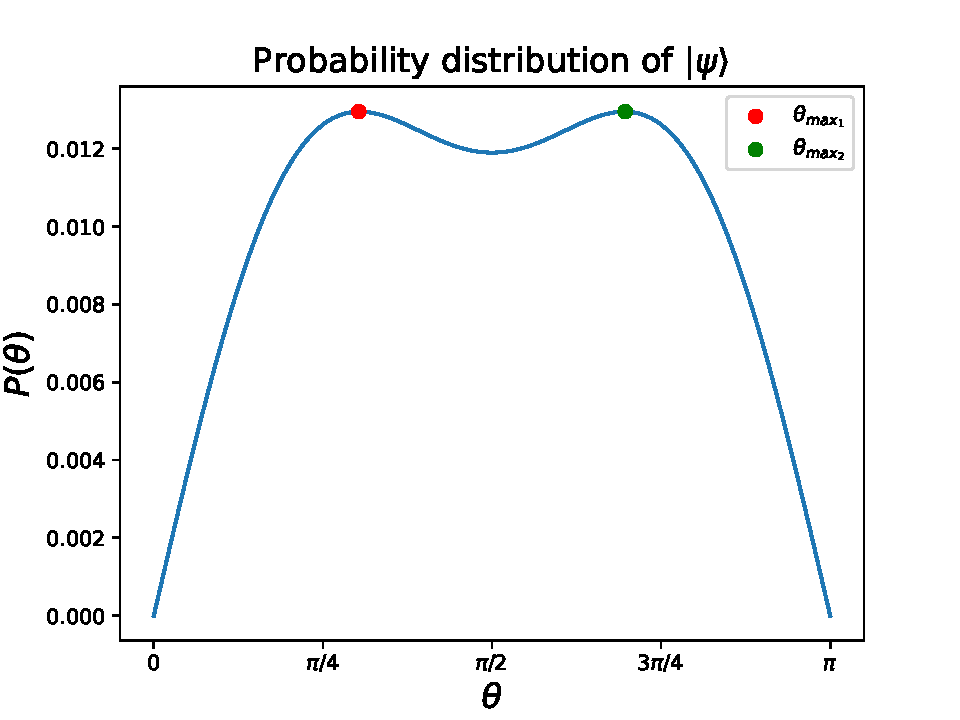
\includegraphics[width = .65\textwidth]{g.pdf}
\caption{Probability distribution of the possible angles the particle could have to the $z$-axis}
\label{fig: g}
\end{figure}

\section*{h)}
We begin by expressing the angular momentum operators in terms of the position and momentum operators:

% \boks{
%   \begin{align}
%     \hat{X}             &= x\\
%     \hat{Y}             &= y\\
% \hat{L}_z           &= xp_y - yp_x\\
% \hat{L}^{†}_z          &= \hat{L}_z\\
% \hat{P}_x           &= -iℏ\frac{∂}{∂x}\\
% \hat{P}_y           &= -iℏ\frac{∂}{∂y}\\
% \left[\hat{X},\hat{P}_x\right] &= iℏ\\
% \left[\hat{Y},\hat{P}_y\right] &= iℏ
% \end{align}
% }

\boks{
  \subsection*{Definitions and Relations:}
\begin{equation*}
\begin{aligned}[c]
\hat{X}    &= x\\
\hat{Y}    &= y\\
\hat{L}_z  &= xp_y - yp_x\\
\hat{L}^{†}_z &= \hat{L}_z\\
\end{aligned}\quad \vline \quad 
\begin{aligned}[c]
\hat{P}_x           &= -iℏ\frac{∂}{∂x} = p_x \\
\hat{P}_y           &= -iℏ\frac{∂}{∂y} = p_y \\
\left[\hat{X},\hat{P}_x\right] &= iℏ\\
\left[\hat{Y},\hat{P}_y\right] &= iℏ
\end{aligned}
\end{equation*}
}

    
\subsection*{$\bf\underline{\left[\hat{L}_z, \hat{P}_x\right]}:$}
\begin{align}
\left[\hat{L}_z, \hat{P}_x\right] = \left[xp_y - yp_x, p_x\right]
\end{align}
\begin{align}
\Big(xp_yp_x - yp_xp_x\Big) - \Big(p_x x p_y - p_x y p_x\Big)
\end{align}
\begin{align}
x p_y p_x - p_x x p_y
\end{align}
\begin{align}
\left[\hat{X}\hat{P}_y, \hat{P}_x\right] = \hat{X} \underbrace{\left[\hat{P}_y, \hat{P}_x\right]}_{0} + \underbrace{\left[\hat{X}, \hat{P}_x\right]}_{iℏ}\hat{P}_y
\end{align}
\begin{align}
\underline{\underline{\left[\hat{L}_z, \hat{P}_x\right] =  iℏ\hat{P}_y}}
\end{align}

\subsection*{$\bf\underline{\left[\hat{L}_z, \hat{P}_y\right]}:$}
\begin{align}
\left[\hat{L}_z, \hat{P}_y\right] = \left[xp_y - yp_x, p_y\right]
\end{align}

\begin{align}
\Big(x p_y p_y - y p_x p_y\Big) - \Big(p_y x p_y - p_y y p_x\Big)
\end{align}
\begin{align}
p_y y p_x - y p_x p_y
\end{align}
\begin{align}
\left[\hat{P}_y, \hat{Y}\hat{P}_x\right] = \underbrace{\left[\hat{P}_y, \hat{Y}\right]}_{-[\hat{Y},\hat{P}_y]}\hat{P}_x + \hat{Y}\underbrace{\left[\hat{P}_y, \hat{P}_x\right]}_{0}
\end{align}
\begin{align}
\underline{\underline{\left[\hat{L}_z, \hat{P}_y\right] = -iℏ\hat{P}_x}} 
\end{align}

\subsection*{Acting on States:}
\subsubsection*{$\hat{P}_x$:}
Checking under which conditions $\bra{l',m'}\hat{P}_x\ket{l,m} = 0$
\begin{align}
\bra{l',m'}\hat{P}_x\ket{l,m} = -\frac{1}{iℏ} \bra{l',m'}\left[\hat{L}_z, \hat{P}_y\right]\ket{l,m}
\end{align}
Expanding the commutator and rewriting the fraction, we get:
\begin{align}
\frac{i}{ℏ}\bra{l',m'}\left(\hat{L}_z \hat{P}_y - \hat{P}_y \hat{L}_z\right)\ket{l,m}
\end{align}
We apply the first angular momentum operator on the bra, and the second on the ket:
\begin{align}
i\bra{l',m'}\left(m' \hat{P}_y - m \hat{P}_y\right)\ket{l,m}
\end{align}
For the expression to be zero, we must have $m' = m$. We take out this factor and keep going:
\begin{align}
i(m'-m) \bra{l',m'}\hat{P}_y\ket{l,m}
\end{align}
Again we replace the momentum operator with the commutator:
\begin{align}
i(m'-m) \frac{1}{iℏ} \bra{l',m'}\left[\hat{L}_z, \hat{P}_x\right]\ket{l,m}
\end{align}
We expand the commutator and rewrite the fraction:
\begin{align}
\frac{1}{ℏ} (m' - m) \bra{l',m'}\left(\hat{L}_z \hat{P}_x - \hat{P}_x \hat{L}_z\right)\ket{l,m}
\end{align}
We apply the first angular momentum operator on the bra, and the second on the ket:
\begin{align}
(m' - m) \bra{l',m'}m'\hat{P}_x - m \hat{P}_x\ket{l,m}
\end{align}
\begin{align}
(m' - m)^2 \bra{l',m'}\hat{P}_x\ket{l,m} 
\end{align}
We clearly see that were back where we started. We can set up the following equation:
\begin{align}
(m' - m)^2 \bra{l',m'}\hat{P}_x\ket{l,m} = \bra{l',m'}\hat{P}_x\ket{l,m}
\end{align}
For this to be true without $\bra{l',m'}\hat{P}_x\ket{l,m}$ being zero, we must have:
\begin{align}
(m' - m)^2 = 1
\end{align}
This gives us two possible values for $m'$:
\begin{align}
m' = m ± 1
\end{align}
\underline{\underline{This shows that $\bra{l',m'}\hat{P}_x\ket{l,m} = 0$ for $m' ≠  m ±1$}}

\subsubsection*{$\hat{P}_y$:}
Checking under which conditions $\bra{l',m'}\hat{P}_y\ket{l,m} = 0$
\begin{align}
\bra{l',m'}\hat{P}_y\ket{l,m}
\end{align}
Again replacing the operator with the commutator:
\begin{align}
\frac{1}{iℏ} \bra{l',m'}\left[\hat{L}_z, \hat{P}_x\right]\ket{l,m}
\end{align}
\begin{align}
\frac{1}{iℏ} \bra{l',m'}\left(\hat{L}_z \hat{P}_x - \hat{P}_x \hat{L}_z\right)\ket{l,m}
\end{align}
We apply the first angular momentum operator on the bra, and the second on the ket, and factor out the $m$ and $m'$-values:
\begin{align}
-i(m'-m) \bra{l',m'}\hat{P}_x\ket{l,m}
\end{align}
We replace the momentum operator with the commutator:
\begin{align}
-i(m'-m) \frac{-1}{iℏ} \bra{l',m'}\left[\hat{L}_z, \hat{P}_y\right]\ket{l,m}
\end{align}
Expanding the commutator, applying the angular momentum operators and factoring out the $m$ and $m'$-values, we get:
\begin{align}
(m'-m)^2 \bra{l',m'}\hat{P}_y\ket{l,m} 
\end{align}
Again we see we are back were we started can set up the following equation:
\begin{align}
(m'-m)^2 \bra{l',m'}\hat{P}_y\ket{l,m} = \bra{l',m'}\hat{P}_y\ket{l,m}
\end{align}
\begin{align}
m' = m ± 1
\end{align}
\underline{\underline{Agin we get the same solution of the $\bra{l',m'}\hat{P}_x\ket{l,m}$ being zero for $m' ≠  m ±1$.}}

\subsubsection*{$\hat{P}_z$:}
Checking under which conditions $\bra{l',m'}\hat{P}_z\ket{l,m} = 0$. We already know that $\left[\hat{L}_z, \hat{P}_z\right] = 0$. Therefore, the following:
\begin{align}
\bra{l',m'}\left[\hat{L}_z, \hat{P}_z\right]\ket{l,m} = 0
\end{align}
Must also be true. Expanding the commutator we get:
\begin{align}
\bra{l',m'}\left(\hat{L}_z \hat{P}_z  - \hat{P}_z \hat{L}_z \right)\ket{l,m}
\end{align}
We apply the first angular momentum operator on the bra, and the second on the ket:
\begin{align}
ℏ(m'-m) \bra{l',m'}\hat{P}_z\ket{l,m}
\end{align}
\underline{\underline{For this to still be zero, we must have $m' = m$.}}. 

\section*{i)}
\begin{align}
\hat{H}_e = \frac{γ}{ℏ}i \left(\hat{L}_z \hat{L}_y - \hat{L}_y \hat{L}_z\right)
\end{align}
\begin{align}
\hat{H}_e = \frac{γ}{ℏ}i [\hat{L}_z, \hat{L}_y]
\end{align}
We know the commutation relation $[\hat{L}_y, \hat{L}_z] = i ℏ \hat{L}_x$. Switching places when commuting, switches the sign, and thus we can write:
\begin{align}
\hat{H}_e = -ii\frac{γ}{ℏ} ℏ \hat{L}_x
\end{align}
\begin{align}
\hat{H}_e = γ \hat{L}_x
\end{align}
Adding this to the total Hamiltonian, we get:
\begin{align}
\hat{H} = \frac{α}{ℏ} \vec{L}^2 + β \hat{L}_z + γ \hat{L}_x
\end{align}
Applying the added term on an arbitrary eigenstate $\ket{m,l}_x$ we get:
\begin{align}
\hat{L}_x \ket{m,l}_x = m ℏ \ket{m,l}_x
\end{align}
The total energy eigenvalues could be written as:
\begin{align}
E_{l,m} = α ℏl(l+1) + β ℏ m_z + γ ℏ m_x
\end{align}
This does not make sense as the particles can't be measured to have angular momentum in both the $x$ and $z$ direction at the same time. We should therefore modify the expression to reflect how the magnetic field affects the components of the angular momentum. One could write one Hamiltonian for calculation along the $x$ and $z$-axis each, but this would be unpractical if you were to measure the angular momentum in a different direction. We can therefore write the Hamiltonian as a function of the direction $\hat{u}$ the measurement is taking place. This could be expressed like this:
\begin{align}
\underline{\underline{H = \frac{α}{ℏ} \vec{L}^2 + \hat{u} ⋅ \vec{B}\ L_u}}
\end{align}
Where $\hat{u}$ is the unit vector in the direction of the measurement, and $\vec{B} = (γ, 0, β)$, representing the field strength in the $x$, $y$ and $z$-direction respectively. $L_u$ is the angular momentum in the direction of the measurement, with eigenvalues $\pm m_u ℏ$ \& $0$ for $m_u ∈ [-l,l] ⋂ ℤ $. The possible eigenvalues of this equation are therefore:
\begin{align}
\underline{\underline{E = α ℏl(l+1) + \hat{u} ⋅ \vec{B}\ m_u ℏ}}
\end{align}


\subsection*{Examples of Acting on States in Different Directions:}
\subsubsection*{$x$-direction}
\begin{align}
\hat{H} \ket{1,1}_z &= \frac{α}{ℏ} \vec{L}^2 \ket{1,1}_z + \hat{z} ⋅ \vec{B}\ L_z \ket{1,1}_z \\
&= \underline{2αℏ + β ℏ }
\end{align}

\subsubsection*{$z$-direction}
\begin{align}
\hat{H} \ket{1,-1}_x &= \frac{α}{ℏ} \vec{L}^2 \ket{1,1}_x + \hat{x} ⋅ \vec{B}\ L_x \ket{1,1}_x \\
&= \underline{2αℏ - γ ℏ}
\end{align}

\subsubsection*{Intermediate Direction}
This notation also allow us to act on states in other directions, like $45^∘$ between the $x$ and $z$-axis:
\begin{align}
r = (1, 0, 1)
\end{align}
\begin{align}
\hat{H} \ket{1,1}_r &= \frac{α}{ℏ} \vec{L}^2 \ket{1,1}_r + \hat{r} ⋅ \vec{B}\ L_r \ket{1,1}_r \\
&= \underline{2αℏ + \frac{1}{\sqrt{2}} (γ + β) ℏ}
\end{align}

\end{document}